\chapter{Dienste}
\label{cha:dienste}
Die Dienstübersicht zeigt alle zukünftigen Dienste absteigend sortiert nach Datum. Jeder Dienst wird als Block klar getrennt und übersichtlich dargestellt. In Abbildung \ref{fig:view_service} \textit{\nameref{fig:view_service}} ist ein einzelner Dienst exemplarisch abgebildet.

\begin{figure}[h]
 \begin{addmargin}{-0.2\linewidth}
   \centering 
   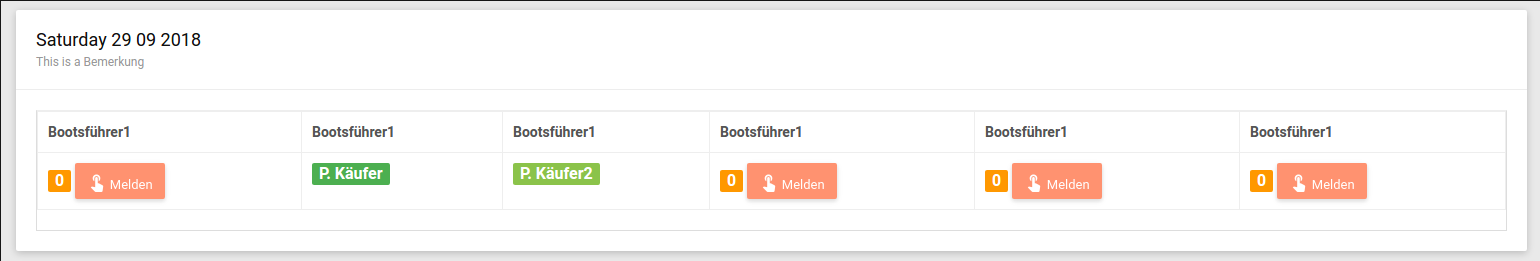
\includegraphics[width=20cm]{Bilder/view_service.png}
 \end{addmargin} 
 \caption[Dienste Übersicht]{DLRG Dienstplan Dienste Übersicht}
 \label{fig:view_service}
\end{figure}

\noindent Jeder Dienst ist mit Tag und Datum beschriftet. Darunter kann eine Bemerkung bzw. Beschreibung hinterlegt sein. Die einzelnen Positionen des Dienstes werden als Tabelle dargestellt.
\noindent Dem Benutzer kann eine Position in fünf verschiedenen Ansichten präsentiert werden mit welchen er zum teil Interagieren kann.
Diese sind in der folgenden Tabelle aufgezeigt und Beispiele beziehen sich immer auf \ref{fig:view_service} \textit{\nameref{fig:view_service}}

\begin{itemize}
\item Melden (bsp. Position 4): Für diese Position ist noch nicht zugeteilt und der Benutzer kann sich hierzu melden.
\item Melden deaktiviert (bsp. Position 1): Für diese Position ist noch nicht zugeteilt. Der Benutzer hat aber nicht die entsprechende Qualifikation.
\item Position bestätigt (bsp. Position 2): Die Position ist bereits zugeordnet.
\item Position bestätigt (bsp. Position 3): Diese Position ist an den Benutzer zugeordnet. Alle zugeordneten Positionen des eigenen Benutzers werden zur besseren Übersicht hellgrün dargestellt.
\item Für Position gemeldet, noch nicht bestätigt (bsp. Position 5): Für diese Position hat der Benutzer sich bereits gemeldet. Solange dies durch die Administratoren noch nicht bestätigt ist, kann die Meldung zurück gezogen werden.
\end{itemize}

\noindent Die Zahl in den Orangenen Kästen vor dem Melde Button (bsp Position 4) gibt an, wie viele andere Benutzer sich bereits für diese Position gemeldet haben. Ein Benutzer kann sich für beliebig viele Positionen eines Dienstes melden. Ebenso können beliebig viele Benutzer sich für eine Position melden. Durch die Administratoren wird nur einer Benutzer für eine Position bestätigt.

\noindent Positionen können Kommentare beinhalten (bsp. Position 1). Mit Kommentaren können geteilte Positionen (Position 1 nur bis 14 Uhr) realisiert werden. Des weiteren können mit Kommentaren auch auf Besonderheiten zu dieser Position hingewiesen werden.